\chapter{Host company and Project context}

\renewcommand{\chaptername}{Chapter}

\section*{Introduction}

This chapter is reserved to present STILL GmbH as the host company, its organizational structure, the mother 
company KION group. It will then proceed to describe the range of products that the company produces.
The second part is dedicated to set the project context by explaining the problem statement, the motivation 
behind this thesis project, and its specifications.
The final part will emphasize the work methodology adopted to carry out this project.

\begin{sloppypar}
\section{Host company: STILL GmbH}
\end{sloppypar}

This section introduces the host group and company through their activities, products, and activities

\subsection{KION Group and STILL GmbH}

STILL GmbH, based in Hamburg, Germany, is a leading manufacturer of intralogistics solutions with 14 locations 
in Germany and a global sales network spanning 246 locations. 
Operating under the KION Group, Europe’s largest forklift truck manufacturer, STILL boasts over 100 years of 
experience. The company develops highly efficient, client-tailored products, serving businesses of all sizes 
with a wide range of forklift trucks—from manually driven forklifts to high-reach trucks and fully automated 
vehicles—alongside consultancy services and software solutions. 

STILL prioritizes smart logistics and energy optimization while maintaining award-winning product quality, 
catering to industries such as food and retail, automotive, and electronics. Employing over 9,000 people across 
departments like sales and marketing, research and development, production, mechatronics, and quality assurance, 
STILL remains at the forefront of intralogistics innovation. 

KION Group is one of the global leaders in the fields of industrial trucks and supply chain solutions.
It is the mother company of: Linde, Dematic Baoli, OM, Fenwick, and STILL who produce the goods and services of the group as 
detailed in Figure \ref{KION Segments}. 

Present in 4 continents and hiring more than 42000 employees, KION's startegy is to ensure profitable ans sustainable growth 
while focusing on Automation and robotics deplyment as one of the main leaders of this growth. 

\begin{figure}[H]
    \begin{center}
     % Requires \usepackage{graphicx}
    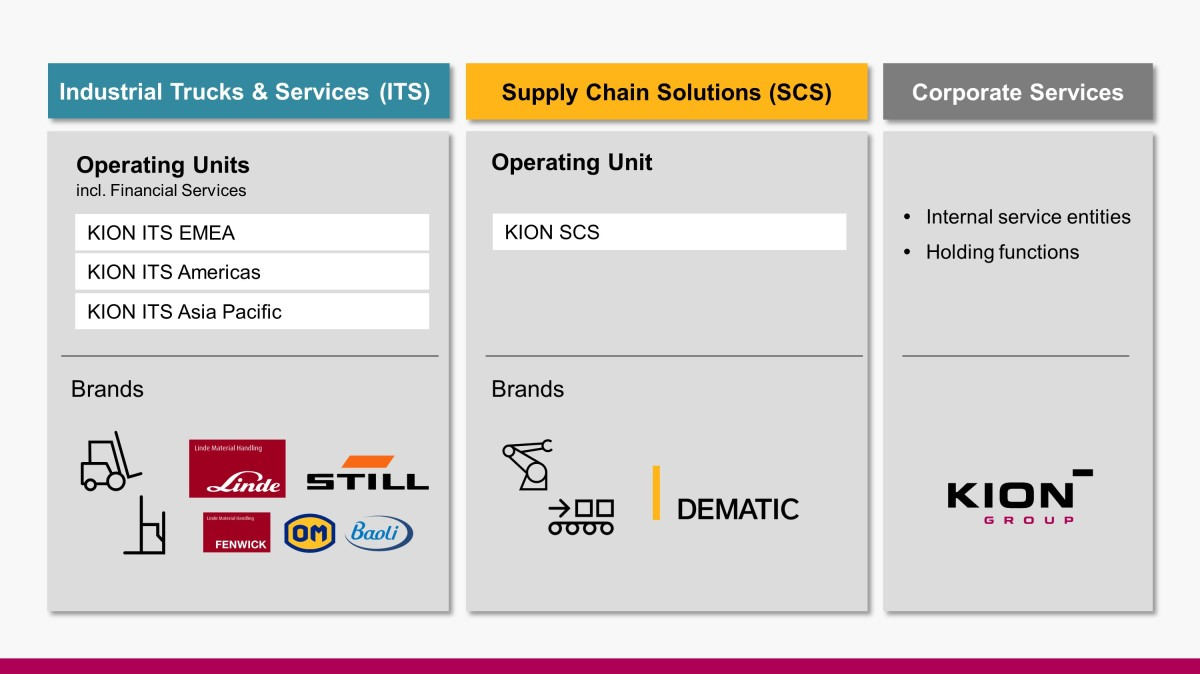
\includegraphics[width=5in]{images/Chap0/KION_Segments.jpg}\\
    \caption{KION segment services and companies \cite{R1}}
    \label{KION Segments}
    \end{center}
    \end{figure}

    
\subsection{KION Management Hierarchy}

The company is composed of departments managing the operations in all companies that are divided by scope of 
interest like R\&D, Management, finances, etc.. Figure \ref{KION Hierarchy} illustrates the different areas of 
responsibility of the Executive
Board. The Autonomous vehicles team belongs to the Mobile Automation department under CTO. 

\subsection{STILL Products}

The 2017-established Autonomous vehicles team aims to develop fully automated solutions that leverage 
novel technologies to create innovative services delivered through forklift trucks. 
The vehicles are developed while keeping safety and high-performance as the main priorities.  

iGo neo shown in Figure \ref{iGoNeo} is one of the main products developed by the department, it is a low level order picker transformed 
into the agent's autonomous assistant. Functioning in autonomous or semi-autonomous modes, it can follow 
the operator and their pace while avoiding obstacles and perceiving their surroundings as well as pick 
and place pallets in designed areas. Its added value is in preserving ergonomics of the operators by 
preventing heavy load carrying for long distances and decreasing the driving ascents and descents by 75\% 
thus increasing the personal and collective performances \cite{R3}.

\begin{figure}[H]
    \begin{center}
     % Requires \usepackage{graphicx}
    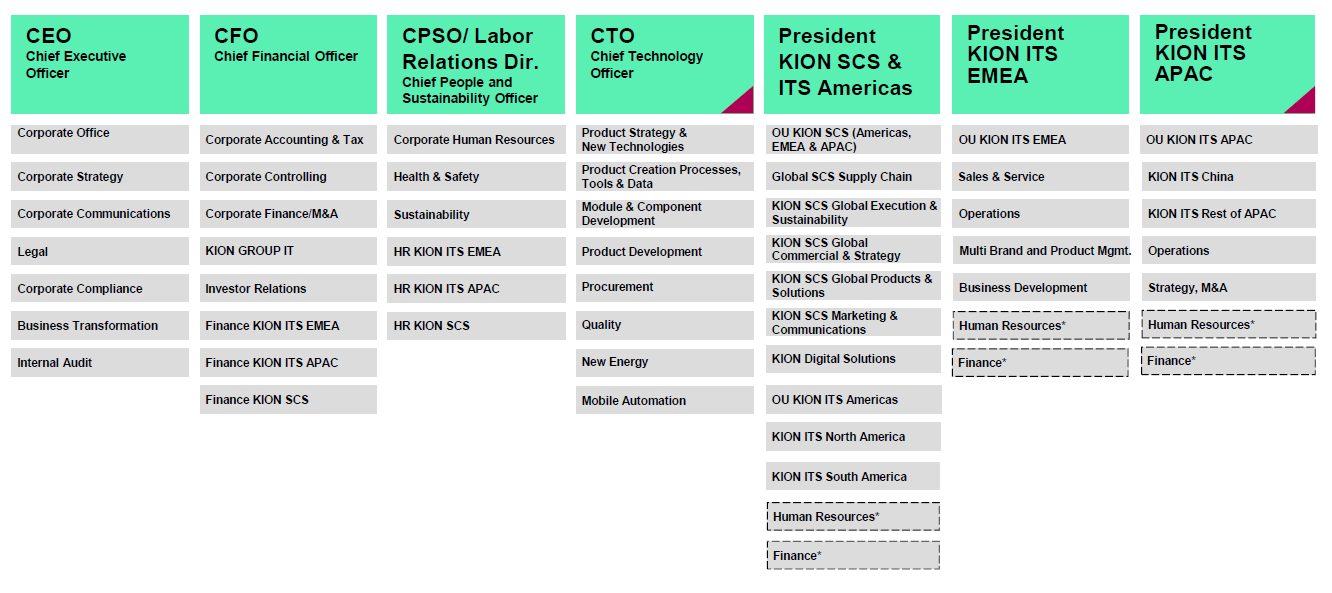
\includegraphics[width=\linewidth]{images/Chap0/KION_Hierarchy.png}\\
    \caption{KION Executive Board responsibilities as of 01.2024 \cite{R2}}
    \label{KION Hierarchy}
    \end{center}
    \end{figure}

As STILL specializes in forklift trucks, it counts many other products. Trucks are either Diesel or 
Gas fueled, or electric trucks that use Li-Ion batteries. Depending on the client's warehouse type, they can
choose from a vast range of reach trucks Figure \ref{Reach trucks}, hand pallet trucks Figure \Ref{hand truck}, 
double stacker trucks Figure \Ref{double-}, and Automated industrial Trucks Figure \Ref{iGoNeo} \cite{R4}.


\begin{figure}[h!]
    \centering
    \begin{minipage}{0.45\textwidth}
        \centering
        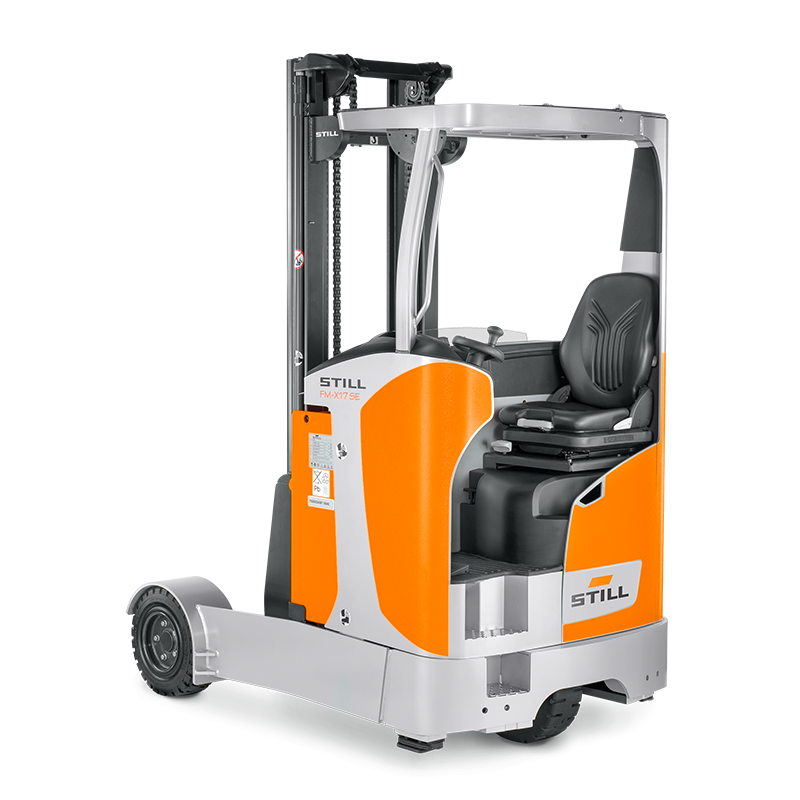
\includegraphics[width=\linewidth]{images/Chap0/Reach trucks.png} % Replace with your figure
        \caption{STILL tractor}
        \label{Reach trucks}
    \end{minipage}
    \begin{minipage}{0.45\textwidth}
        \centering
        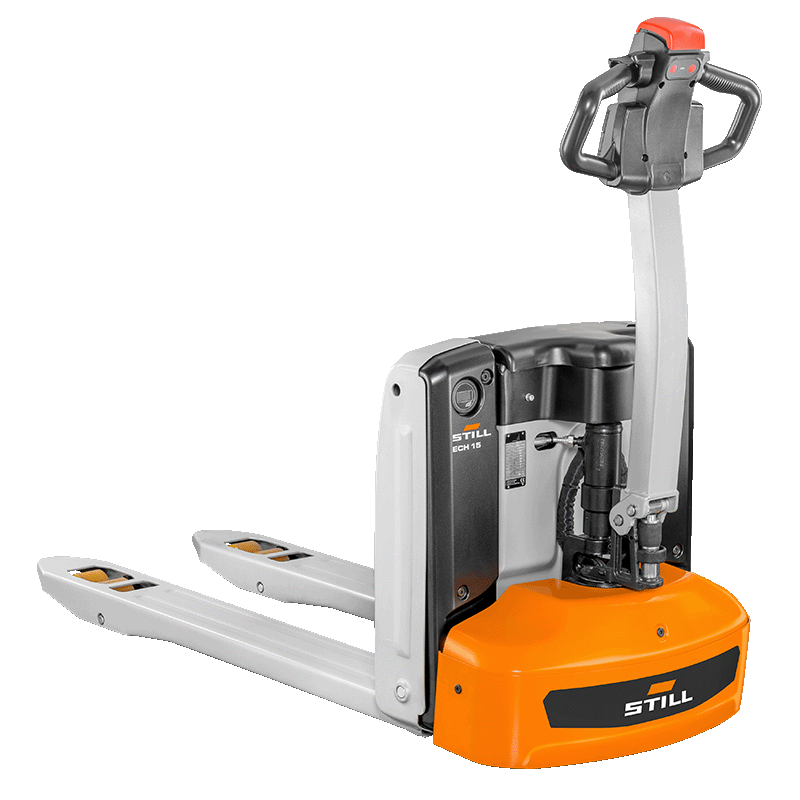
\includegraphics[width=\linewidth]{images/Chap0/hand truck.png} % Replace with your figure
        \caption{STILL hand truck}
        \label{hand truck}
    \end{minipage}
\end{figure}

\begin{figure}[H]
    \centering
    \begin{minipage}{0.45\textwidth}
        \centering
        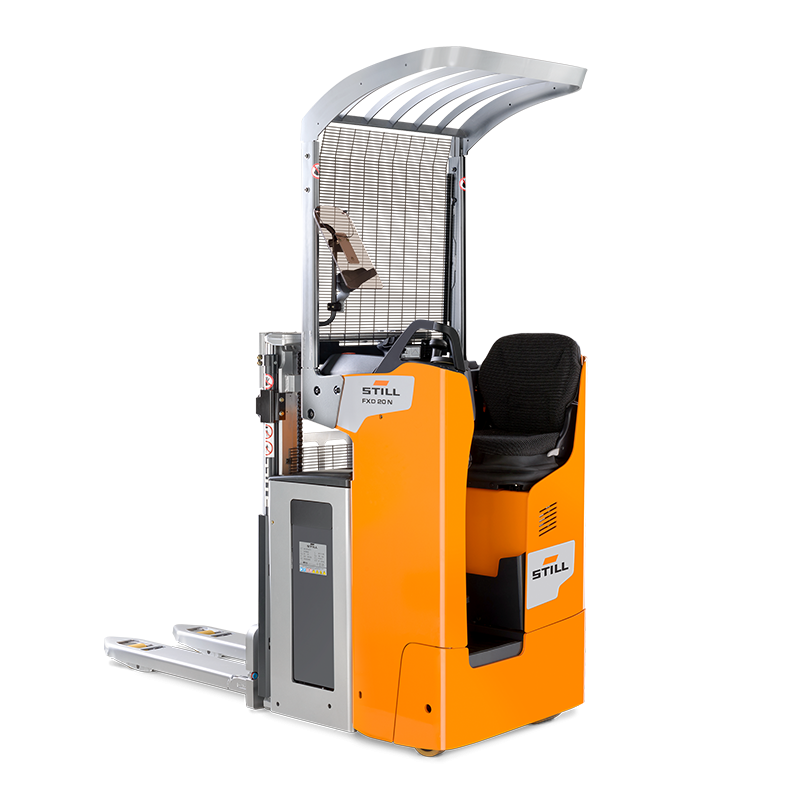
\includegraphics[width=\linewidth]{images/Chap0/double-.png} % Replace with your figure
        \caption{STILL rider truck}
        \label{double-}
    \end{minipage}
    \begin{minipage}{0.45\textwidth}
        \centering
        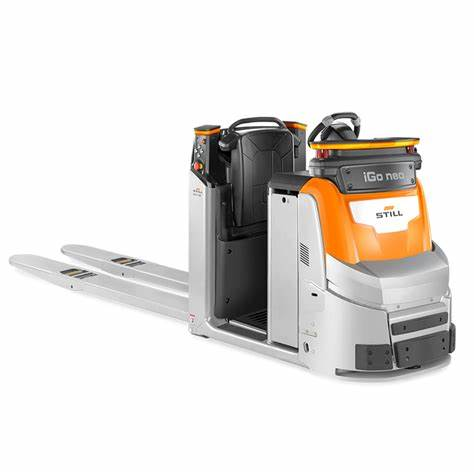
\includegraphics[width=\linewidth]{images/Chap0/iGoNeo.jpg} % Replace with your figure
        \caption{STILL iGo neo}
        \label{iGoNeo}
    \end{minipage}
\end{figure}

Despite the impressive capabilities of the iGo neo and similar autonomous vehicles, the implementation 
of such advanced technology brings up several challenges, particularly in ensuring reliable and predictable 
behavior under all operating conditions. This leads to a key motivation for further investigation and improvement 
in the field.

\section{Graduation project Motivation and Problem Statement}

\subsection{Motivation}


While autonomous vehicles can be highly reliable and efficient in carrying out various 
tasks, their behavior is not always predictable or easily explained. The output often 
exhibits a stochastic nature. For example, an obstacle-avoiding solution planned by 
the autonomous vehicle may be safe and correct but might follow an unusually shaped path. 

Such stochastic behaviors can lead to a lack of trust and interest in robotized forklift 
trucks from a customer’s perspective. This unpredictability can cause customers to 
question the system's repeatability, fearing that it may not perform consistently in 
critical situations. Moreover, the unexpected nature of these behaviors can make it 
difficult for operators to understand and anticipate the vehicle's actions, further 
reducing confidence. 

Adding to these concerns, many autonomous systems, particularly in the intralogistics 
sector, require significant commissioning efforts before they can be implemented in 
a new environment and begin their service. Whether it's a required software integration, 
sensors installations, or 
measurements, these systems demand substantial time, information and financial investment—three 
crucial resources that we aim to optimize. Innovation in automation should involve 
the development of optimal solutions that are easy to 
commission in a new environment. These so-called "plug-and-play" solutions reduce 
the effort required and allow customers to start benefiting from the autonomous 
features with just the physical truck on-site and available information about the 
warehouse. the rest, is online recognition and processing. This approach 
significantly enhances the impact and convenience of the technology. 

The autonomous vehicles department focuses on creating reliable, efficient, and 
explainable systems to build trust with customers, encouraging adoption of the technology. 
With a focus on explainable AI, the technology becomes more interpretable, helping customers 
understand decision-making processes and increasing their confidence in its safety and reliability.

\newpage
\subsection{Problem statement}

Autonomous navigation is a topic where explainable intelligence can be integrated. 
Robotic forklifts execute missions such as transporting pallets from one place to another: 
picking up or dropping pallets.
The mission is splitted into:
\begin{itemize}
    \item a movement to a source
    \item a pickup
    \item a movement to the destination
    \item a drop
\end{itemize}
The movement to the source or the destination is the movement in figure \Ref{move} where \(station1\) 
is considered the source station that the truck is headed to.
This movement is planned globally and is not the scope of this work. 
Figure \Ref{move} is a section of the model of a real warehouse. In this work,
the interest is around the following items of the model:
\begin{itemize}
    \item Dark Blue outline: walls of the warehouse
    \item Yellow Rectancles marked as stations: Warehouse stations: Actions like picking up or 
    dropping are performed in specific locations inside the warehouse called 
    stations, examples of which are named \(station1\), \(station2\), and \(station3\) on the figure \Ref{move}.
    Each station is designed to support specific warehouse functions and their general mission
    is to facilitate and organize material handling operations. 
    Each station contains a \textbf{shelf} that contains the pallets to be picked or dropped. 
    \item Black rectangles: storage shelves (also called racks), where the  pallets and material are 
    stored. 
    \item Turquoise blue lines: Global paths that connect the stations.
    The truck takes these routes when navigating from a station to the other while avoiding 
    obstacles online if they occur.
    \item Gray rectangles are starting position of the truck around the warehouse. For instance,
    the truck can be placed at these positions before starting its autonomous navigation and 
    task fulfillment.

\end{itemize}

However, the truck arrives at a distant pose from the shelf or pallet,
the distance is clearly seen in figure \Ref{dock}. In addition, its forks are facing the 
wrong direction because driving the truck should happen like the arrow shows on figure \Ref{move} 
to avoid hitting humans or materials with the forks.

The distance is intended because the truck needs a maneuver to make its forks dock (enter) the shelf
as they are the part that picks up or drops the pallet.


The path that involves this maneuver is called the link path that guides the truck to to the pallet or the drop 
pose (the shelf inside the station in figure \Ref{dock}). 

Online linking of the robotic forklift to the goal pallet or location takes place inside
the station. Online linking is mandatory because warehouse areas are subject to constant changes for instance,
shelves can be shifted from their expected
position and dynamic obstacles can show up, but, the vehicle needs precise recognition of the coordinates 
that it will reach. 
Precise recognition allows for correctness of the picking or dropping processes, otherwise, 
the task can fail. Furthermore, the vehicle has to account for the new obstacles and clutter inside 
of the station and avoid collisioning with them when driving to the destination shelf.

\begin{figure}[H]
    \begin{center}
       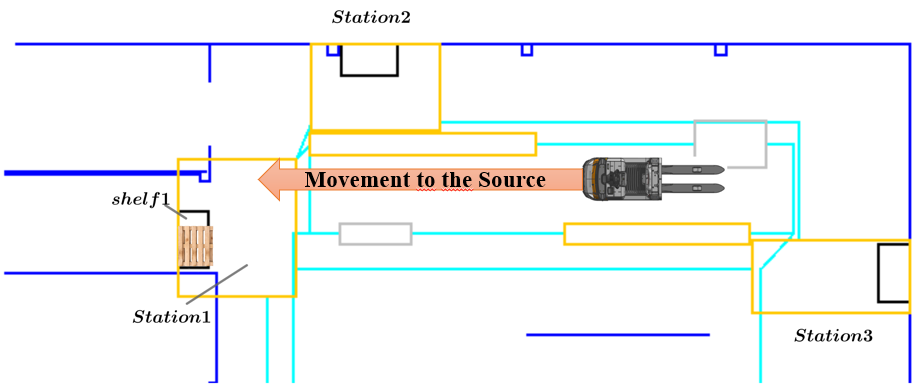
\includegraphics[width=5in]{images/Chap0/move.png}\\
       \caption{Vehicle Moving towards station 1}
       \label{move}
       \end{center}
\end{figure}

\begin{figure}[H]
    \begin{center}
       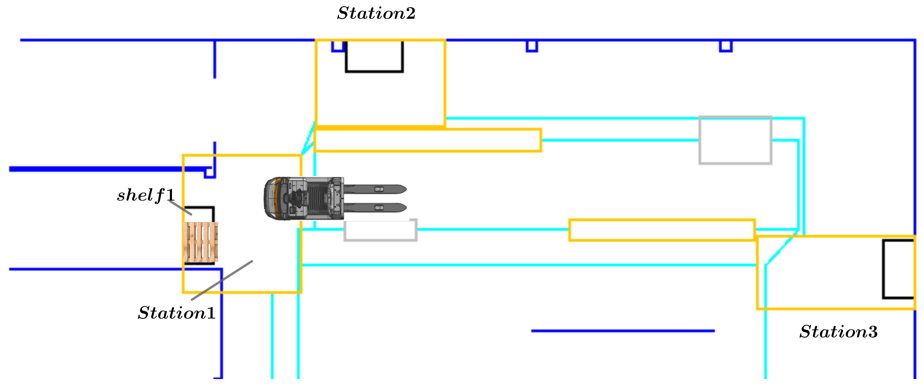
\includegraphics[width=5in]{images/Chap0/arrive.png}\\
       \caption{Vehicle arrives at station 1 and ready to execute the task}
       \label{dock}
       \end{center}
\end{figure}

This thesis focuses on the subtask of an autonoumous online linking of the vehicle to shelf
independantly from the task to be performed (pick up/drop). 
When it arrives at the station, the vehicle is fronted by these constraints:

%TODO: check these
\begin{itemize}
    \item The vehicle’s forks are not facing the destination shelf as shown in figure \Ref{dock} 
    but rather the opposite direction, 
    so a driving direction change is needed. 

    \item The vehicle is bulky in volume and mass (1200 to 4000 kg) with an overall 
    length of 2500 to 4000 mm  \cite{R5}
    which makes it challenging  to change directions: turning on the spot or 
    navigating in highly curved paths. 
    
    \item The pallet docking process has to be very precise to avoid shifts and mistakes. 
\end{itemize}

$\Rightarrow$ \textbf{The goal} is to autonomously and optimally transport the vehicle from the position of entering the station in
figure \Ref{dock_wait} to the position of docking the shelf in figure \Ref{dock_done} while accounting for obstacles,
kinematics of the vehicle, and maximizing speed. 

\begin{figure}[H]
    \begin{center}
    \begin{minipage}[b]{0.6\linewidth}  % First figure is larger (55% of the width)
        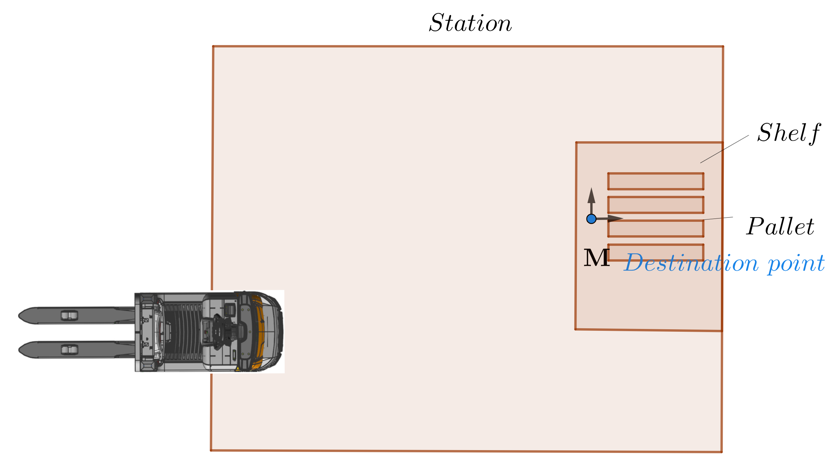
\includegraphics[width=\linewidth]{images/Chap0/dock_wait.png}
        \caption{Vehicle entered the station waiting for docking the shelf}
        \label{dock_wait}
    \end{minipage}
    \hspace{0.02\linewidth}  % Space between the figures (2%)
    \begin{minipage}[b]{0.5\linewidth}  % Second figure is smaller (42% of the width)
        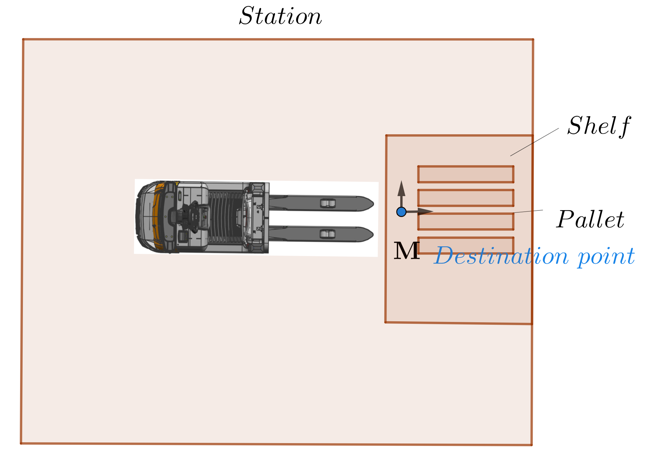
\includegraphics[width=\linewidth]{images/Chap0/dock_done.png}
        \caption{Vehicle docked the shelf}
        \label{dock_done}
    \end{minipage}
    \end{center}
\end{figure}

The next section focuses on the process followed during the development of the project. 

\section{Work Structure and Methodology}

Our team adopts an Agile Scrum methodology showcased in Figure \Ref{Agile Scrum Process} to ensure 
efficient and flexible project management. Here’s how we approach our work:

\begin{figure}[H]
    \begin{center}
       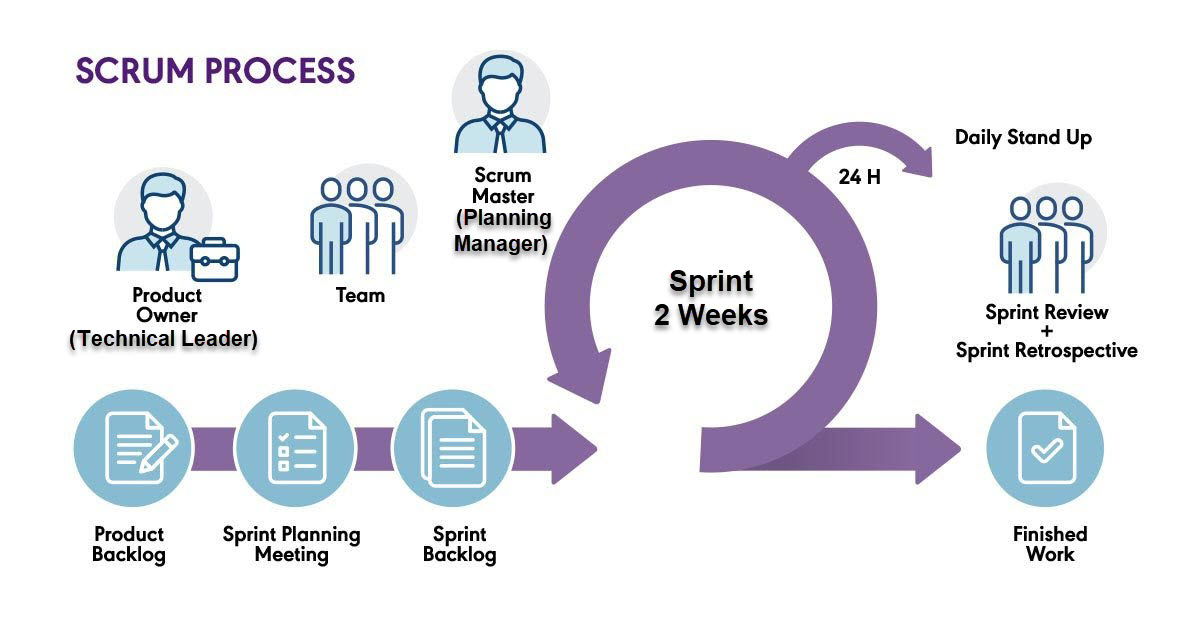
\includegraphics[width=6in]{images/Chap0/blog-scrum-process-opt.jpg}\\
       \caption{Agile Scrum Process \cite{R6}}
       \label{Agile Scrum Process}
       \end{center}
\end{figure}

\subsection{Agile Scrum Framework} 
\begin{itemize}
    \item \textbf{Jira: } We use Jira to organize and track our tasks and progress. Jira allows us to create 
    and manage tickets, which are detailed records of tasks, bugs, or features that need attention. 
    Each ticket is assigned to team members and tracked through its development stages until completion.

    \item \textbf{Sprints: } Our work is organized into 2-week sprints. Each sprint is a focused period 
    where we aim to complete a set of predefined tasks. At the start of each sprint, we hold a meeting to 
    review the previous sprint: every team member presents their completed tickets, and communicates the 
    changes or blockers that appeared during the process and plan for the next sprint: decide which tasks 
    will be tackled during the sprint. 
    This helps us maintain a steady pace and regularly deliver increments of our project.

    \item  \textbf{PI Planning: } Every quarter, we engage in Program Increment (PI) planning with the 
    mobile automation teams. The PI happens in two phases: each team prepares their planning for the next 3
    months, then it is discussed and tailored again in a bigger round. This planning session helps us align 
    our goals and strategies for the upcoming quarter. We review progress, set objectives, and coordinate 
    with other teams to ensure that our work is aligned with broader project goals and company vision.

    \item \textbf{Daily Standups: } We hold 15 minutes long daily standup meetings to keep everyone on the 
    same page. During these meetings, team members share updates on their progress, discuss any challenges 
    they are facing, and outline their plans for the day. This practice promotes transparency, communication and quick 
    problem-solving through collaboration.

\end{itemize}

\subsection{Version Management}
\begin{itemize}
    \item \textbf{GitHub: } We use GitHub for version control and code management. GitHub allows us to 
    collaborate on code, track changes, and manage different versions of our project. Each team member 
    can contribute to the codebase, and we use pull requests to review and integrate new features.
\end{itemize}

\subsection{Communication and Collaboration:}

\begin{itemize}
\item  \textbf{Microsoft Teams: } We use Microsoft Teams for real-time communication and collaboration. 
Teams provides a platform for chatting, video calls, and sharing files, facilitating smooth and efficient 
interactions among team members.

\item  \textbf{Microsoft Outlook: } Outlook is used for email communication and scheduling. It helps us 
manage meetings, track important messages, and coordinate tasks and deadlines.
\end{itemize}

By integrating these tools and practices, we ensure a structured yet flexible workflow, enabling us to adapt to changes, communicate effectively, and deliver high-quality results.